\section{Architecture}
This section describes the software architecture proposed by this project in order to realize the Transparent scheduling model over heterogeneous devices and, consequently, satisfy the requirements and use cases previously described.

\textit{Figure \ref{fig:architecture_complete}} provides a complete view of the Architecture; being a complex project based on the interaction between multiple distributed entities, the schema will be divided in three areas (easier to understand) that will be discussed in the following sections:
\begin{itemize}
    \item Cloud Services area (\textit{section \ref{cloud_services_area}})
    \item Contributor area (\textit{section \ref{contributor_area}})
    \item Customer area (\textit{section \ref{customer_area}})
\end{itemize}
\begin{figure}[!ht]
    \centering
    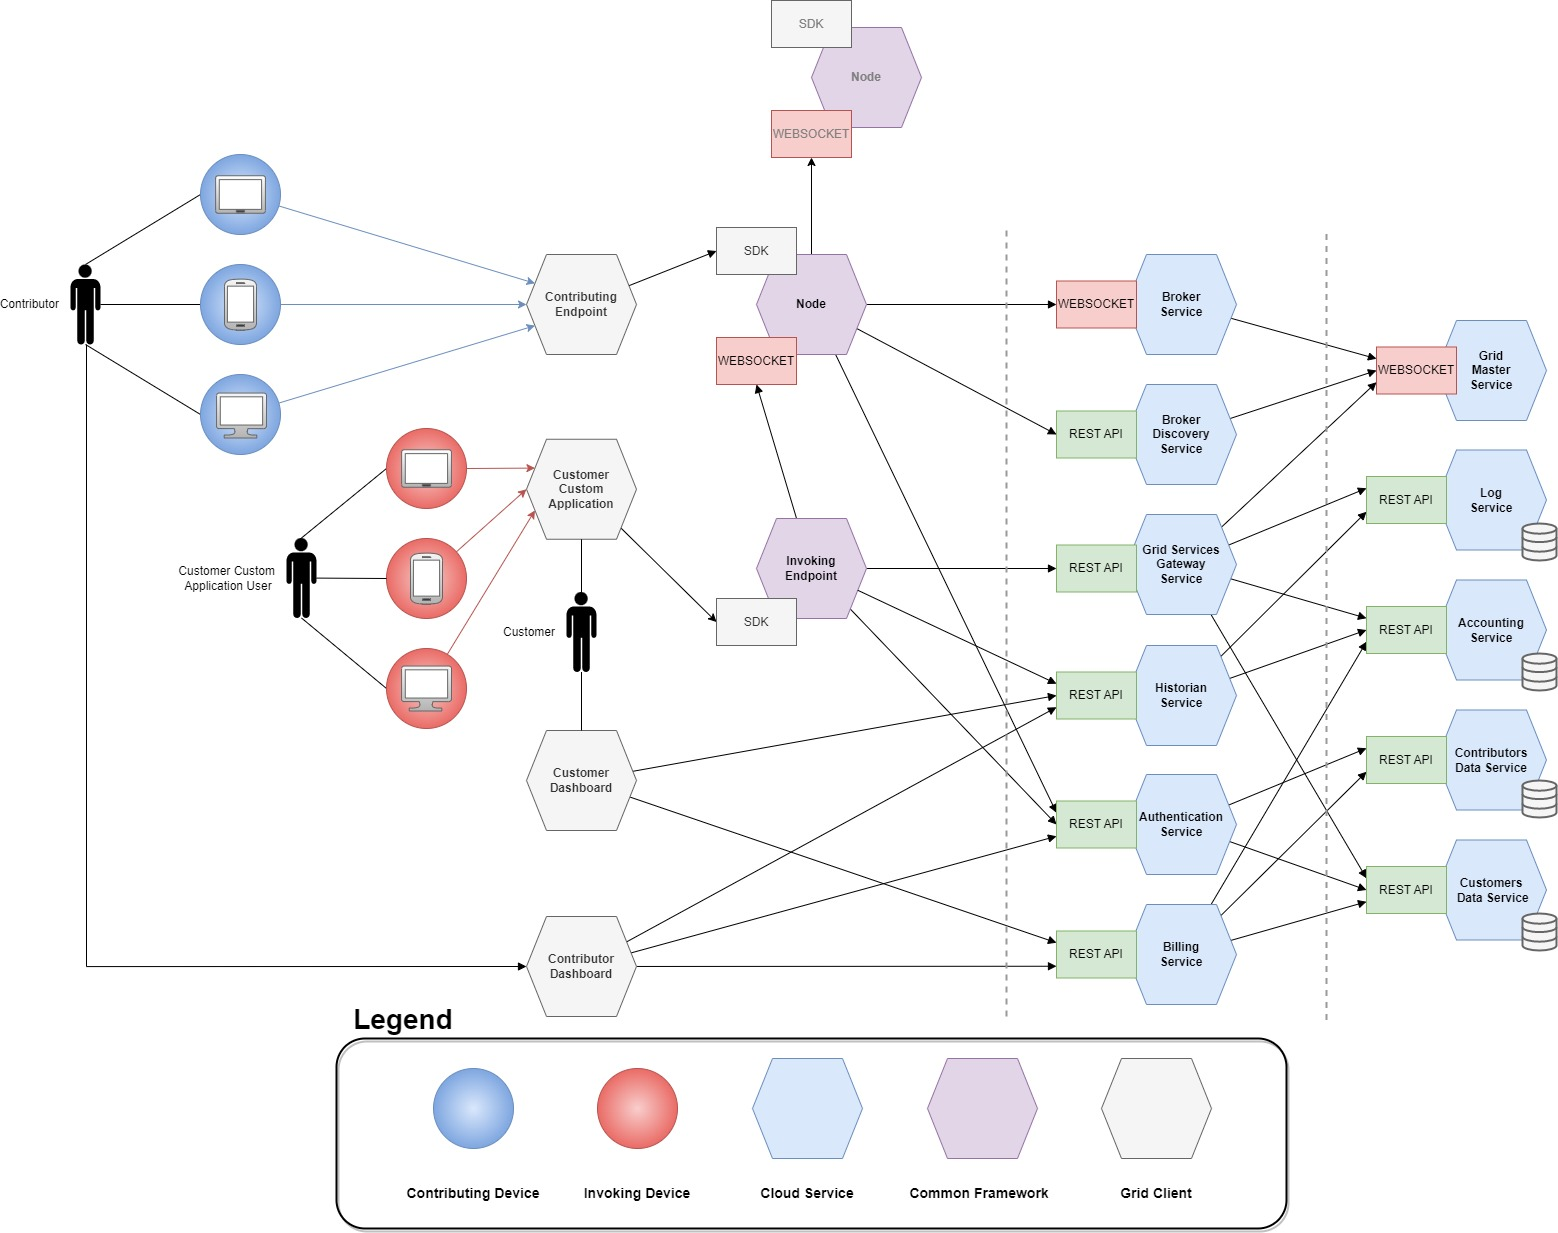
\includegraphics[width=\linewidth]{document/chapters/chapter_6/images/architecture_complete.jpg}
    \caption{Complete view of the Architecture}
    \label{fig:architecture_complete}
\end{figure}

\subsection{Cloud Services Area}\label{cloud_services_area}
The Cloud services follow a Hexagonal architecture composed by a multitude of microservices (\textit{Figure \ref{fig:architecture_cloud_services}}). Each Microservice is accessed through communication interfaces (whether Rest APIs or Web Sockets, depending on the particular microservice needs) and belong to one of the following layers:
\begin{itemize}
    \item \textbf{Business logic}\\
    Microservices that expose core business logic for Grid functionalities realization and data managing. Entities that  reside here are protected, meaning that they are isolated from the outside and their functionalities can only be accessed through the entities placed in the Adapters layer.
    \item \textbf{Adapters}\\
    Microservices that expose functionalities accessed by the entities residing in the Contributor and Customer area; such functionalities are realized through combining the services offered by entities residing in the Business logic layer.
\end{itemize}
\begin{figure}[!ht]
    \centering
    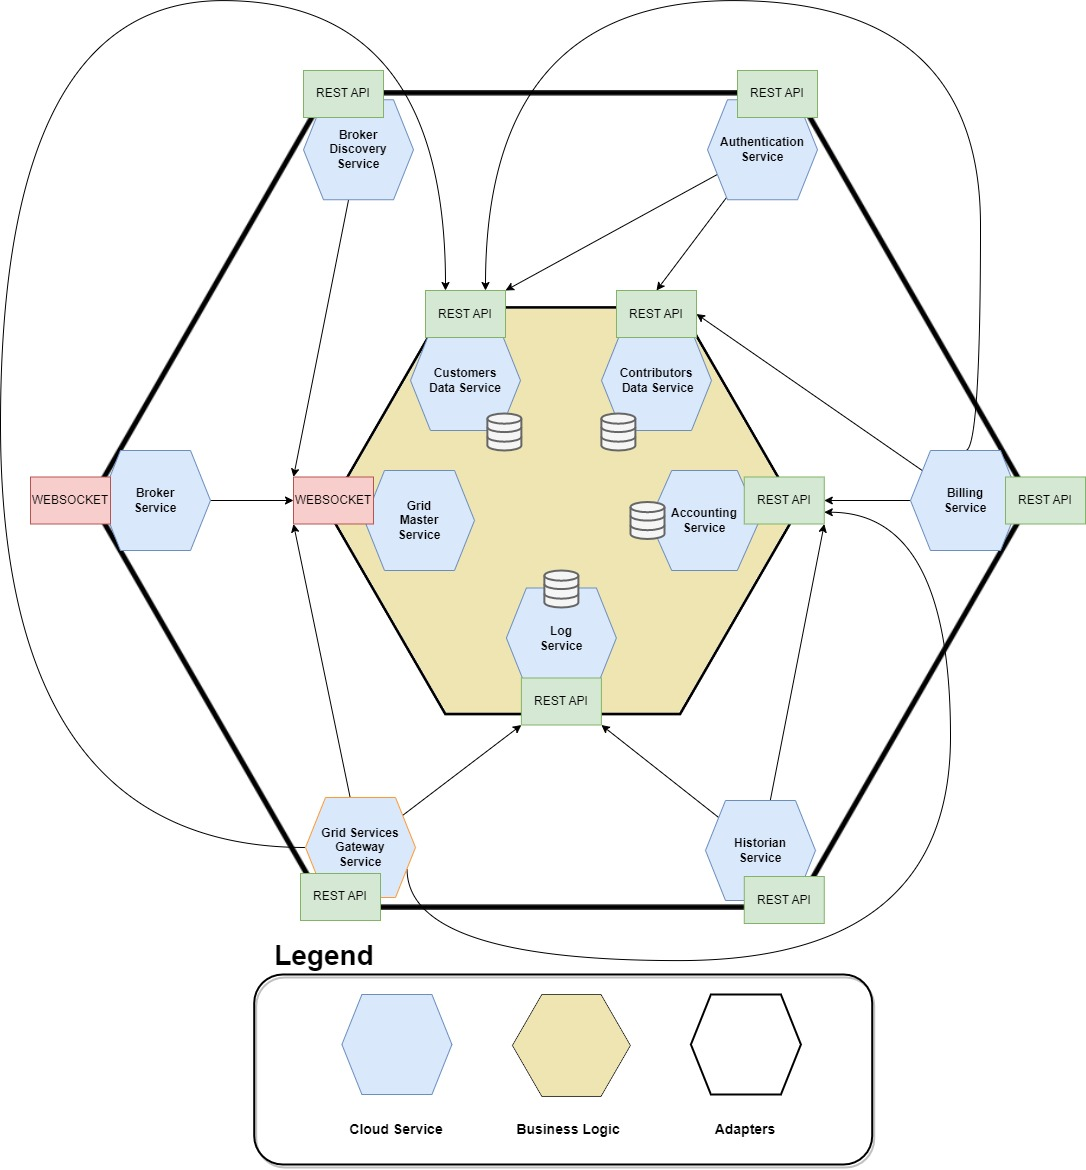
\includegraphics[scale=0.35]{document/chapters/chapter_6/images/architecture_cloud_services.jpg}
    \caption{Architecture: Cloud Services}
    \label{fig:architecture_cloud_services}
\end{figure}

\subsubsection{Business Logic}
\begin{itemize}
    \item \textbf{Grid Master Service}\\
    The main coordinator in the Grid system. It dynamically creates/removes Broker Service instances in order to sustain and balance the traffic generated by Nodes and Invoking Endpoints connected to the current instances of Broker Service; such instances needs to be contacted by Nodes but, being dynamically instantiated, they do not possess a static address. As a consequence of that, the Grid Master Service (that knows such addresses, being the creator of the instances) is connected to the Broker Discovery System (which will provide a Broker Service instance address to a connecting Node).

    \textit{Figure \ref{fig:master_grid_load_balancing}} shows a high level view of the connection between Grid Master, Brokers and Nodes while also providing an example of load balancing. When the new Node [N11] wants to connect to the Grid in order to Contribute, given that no Broker instance is able to handle the Node connection, the Grid Master instantiates [B2] to which [N11] will connect and part of the load handled by [B1] (just [N9] in this example) will be redirected to.
    \begin{figure}[!ht]
        \centering
        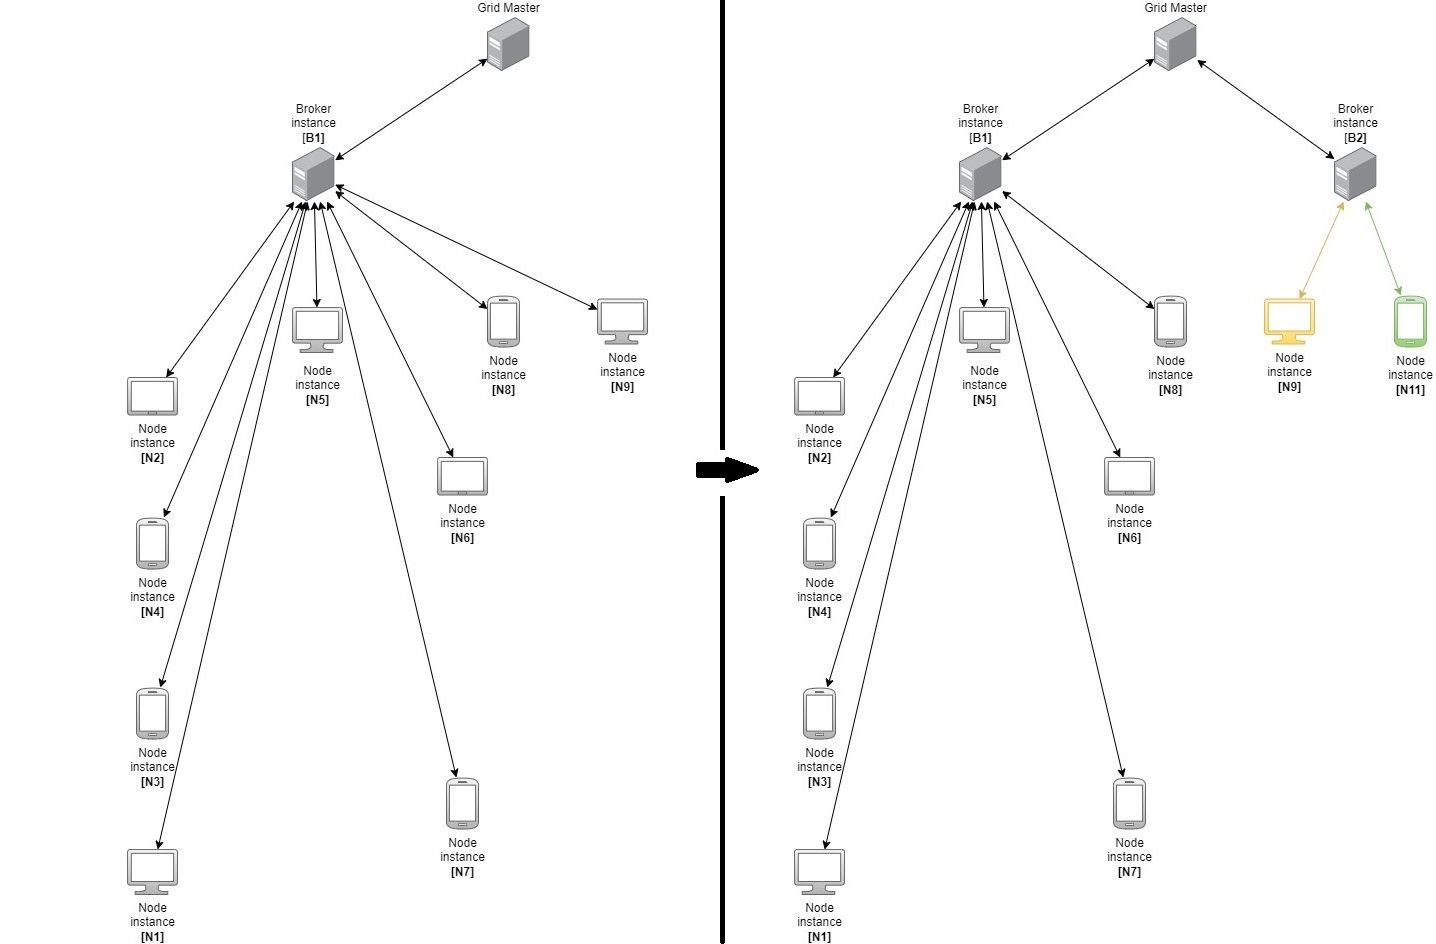
\includegraphics[width=\linewidth]{document/chapters/chapter_6/images/master_grid_load_balancing.jpg}
        \caption{Grid Master Service load balancing}
        \label{fig:master_grid_load_balancing}
    \end{figure}

    Lastly, the Grid Master Service is also connected to the Grid Services Gateway Service; through this last Cloud Service, the Invoking Endpoints request the execution of Grid Services. Thus, the Grid Master (collaborating with the Broker Service instances) will provide the Resources needed to execute the requested Grid Service.

    Concluding, this Cloud Service's importance is vital to the functioning and scalability of the Grid, requiring to expose communication interfaces for the discovery of Brokers, Resources obtainment and Grid coordination.

    \item \textbf{Customer Data Service}\\
    REST server that provides APIs used to read and write data used to uniquely identify a Customer inside the system. It does not contain data about payments or logs about Grid events that involve the Customer since those are handled by the Accounting Service and the Log Service respectively.\\
    Customers are, numerically speaking, considerably less compared to Contributors; this results in less frequent invocations of this Cloud Service's APIs and a far smaller volume of data to persist. Regarding the CAP theorem, it is then important to focus on a database technology that can grant Consistency and Partition Tolerance sacrificing Availability (e.g. MongoDB, BigTable, etc...).

    \item \textbf{Contributor Data Service}\\
    REST server that exposes APIs used to read and write data used to uniquely identify a Contributor and its devices inside the system. The same rules used in the Customer Data Service, regarding the handling of logs and payments data, also hold here; when it comes to the CAP theorem application, on the contrary, this Cloud Service requires AP database technologies (e.g. DynamoDB, Cassandra, etc...).

    \item \textbf{Accounting Service}\\
    REST server exposing APIs to perform and record the history of monetary transactions, involving both Customers and Contributors (i.e. Fees payments and Rewards Redemptions) inside the Grid; Consistency and Partition Tolerance here are key requirements.

    \item \textbf{Log Service}\\
    REST server providing APIs used to read and write unmodifiable logs about Contributions and Grid Services Invocations; this Cloud Service is particularly important to both monitor what is happening inside the Grid and also correctly identify which Node has performed a Contribution and how much of said Contribution it has done. Access speed is the most relevant factor here, making it acceptable to have eventual consistency but not delays; then, AP database technologies are required here. In particular, said AP database technology should use an RDF model (also known as Triplestore) which is particularly suited for log data.
\end{itemize}

\subsubsection{Adapters}
\begin{itemize}
    \item \textbf{Broker Service}\\
    Cloud Service that acts as middleware between the Grid Master and the Nodes (\textit{figure \ref{fig:master_grid_load_balancing}}). There are as many instances as needed to sustain the load of the connections to the Nodes; instances are created and removed by the Grid Master taking in account the geographical location of said Nodes in order to reduce latency for the Broker-Node connection.
    The Broker executes the coordination commands given by the Grid Master while also managing the Nodes connected through its communication channels exposed by its Web Socket.
    
    Let us take, for example, a Grid Service Invocation: the Grid Master contacts a Broker Service instance that is geographically convenient in relationship to the location of the Invoking Endpoint; the Grid Master will delegate to the selected Broker Service instance the responsibility of gathering adequate Resources for the execution of the particular Grid Service requested. The Broker will then spread the request of said Resources to its connected Nodes and gather the responses of the ones that are adequate and available. The Broker will group the info needed to contact such nodes and forward it to the Grid Master that will then be responsible to forward in turn to the requestor.

    \item \textbf{Broker Discovery Service}\\
    This REST server has just one simple responsibility: it provides to a Node the address of a Broker Service in order to make possible a connection between them. This discovery mechanism is necessary since, as already stated, the Broker Service instances are dynamically created and thus they do not possess a static address; on the contrary the Broker Discovery Service will necessarily need a static address known by the Nodes. The trafic directed to this Cloud Service and its computational load tend to be minimal and requires only one instance but, as time goes on and the contributing user base increases, new static instances can be added easily.

    \item \textbf{Grid Services Gateway Service}\\
    In order for Invoking Endpoints to access Resources, they need interact with this REST server; it exposes APIs for a standardized and parameterized access to Resources through the Grid Service abstraction, meaning that a Customer expresses its request in terms of what Grid Service it wants to execute, not in terms of single Resources.
    
    This Cloud Service is connected via Web Socket to the Grid Master Service in order to gather the necessary Resources but, before that, the Grid Services Gateway Service needs to contact the Accounting Service in order to execute the Fee payment. Lastly, the Cloud Service is also connected to the Log Service in order to register the Grid Service invocation and the consequent usage of Resources happened during the computation.

    Similarly to the Broker Discovery Service, the number of static instances easily can vary in the project's lifecycle. 

    \item \textbf{Authentication Service}\\
    Before being able to communicate with any other Cloud Service belonging to the Adapters layer, any entity needs to authenticate to the Grid through this Cloud Service. Given that the two actors that require authentication are the Customer and the Contributor, the Authentication Service utilizes both the Customer Data Service and the Contributor Data Service in its functioning. As a consequence of the authentication, the entity that wants to interact with the Grid will receive a token that uniquely identifies it inside the Grid system.

    \item \textbf{Billing Service}\\
    Cloud Service exposing APIs used to make monetary transactions for Fee payments and Rewards Redemptions. It acts as an intermediary, protecting the actual payment process effectuated by the Accounting Service.
    It does not offer access to info about past monetary transactions, leaving this responsibility to the Historian Service.

    \item \textbf{Historian Service}\\
    The Historian Service exposes APIs that allow the read-only access to event already happened in the Grid System like monetary transactions, Contribution, Grid Services Invocations, etc...

\end{itemize}
\vspace{20mm}

\subsection{Contributor area}\label{contributor_area}
The Contributor area, as shown in \textit{figure \ref{fig:architecture_contributor}}, comprehends three entities:
\begin{itemize}
    \item \textbf{Node}
    \item \textbf{Contributing EndPoint}
    \item \textbf{Contributor Dashboard}
\end{itemize}
The relevant Cloud Services are shown in order to explain the interactions that Node and the Contributor Dashboard have with them; in particular, the Grid Master Service is shown to emphatize the Grid Master - Broker - Node connection seen in \textit{figure \ref{fig:master_grid_load_balancing}}.

Moreover, the Invoking Endpoint (which belongs to the Customer area) and the additional Node instance are included to show the connections that a Node can have with other entities that do not belong to the Cloud Services.

\vspace{5mm}

\begin{figure}[!ht]
    \centering
    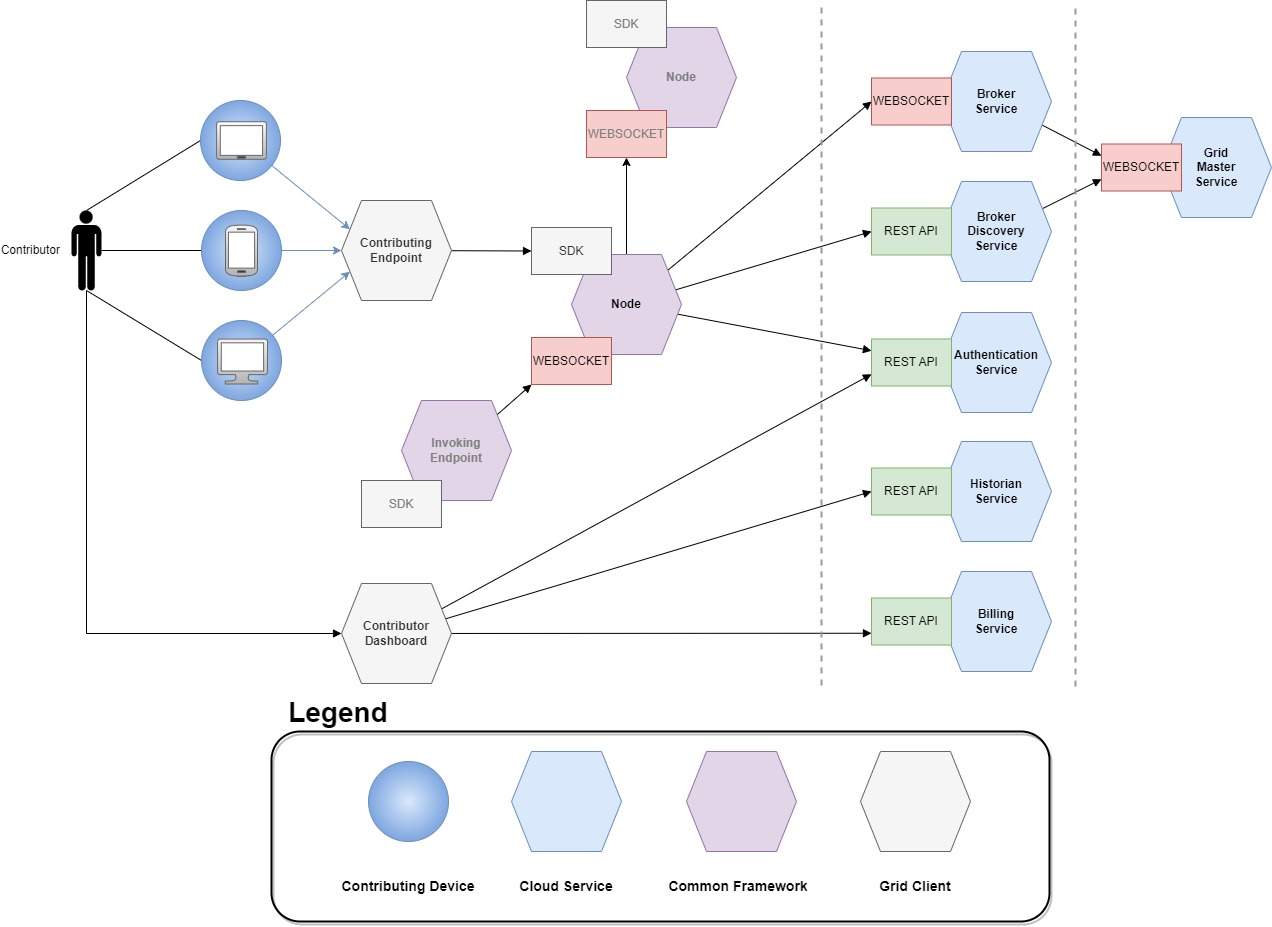
\includegraphics[width=\linewidth]{document/chapters/chapter_6/images/architecture_contributor.jpg}
    \caption{Architecture: Contributor area}
    \label{fig:architecture_contributor}
\end{figure}

\subsubsection{Node}
This is the primary entity when it comes to contribution.
Continuing the definition provided in the Ubiquitous Language (\textit{section \ref{ubiquitous_language}}), this software abstraction is identifiable as a set of core Contribution functionalities and logic which needs to be integrated (through the offered SDK) to an actual software application (Contributing Endpoint) capable of interacting with the specific resources of the device that is running it; thus, a Node exists in order to get a fast integration with as many devices as possible to maximize the compatibility for Contribution, removing the need to reimplement everything for every new Contributing Endpoint.

The model of this solution aims to grant the access to Grid Services also to low-spec devices; thus, it is important to delegate as much work as possible to the Nodes. In order to complete a Grid Service, the Node can Contribute in one of the following ways (depending on the particular Service):
\begin{itemize}
\item \textbf{Direct communication with the Invoking Endpoint}\\
A Node is connected, through a Web Socket, directly to the Invoking Endpoint. Let us take, for example, a hypothetical Grid Service that consists of delegating a computation to a single Node (i.e. non-distributed computation); the Node (Slave) and the Invoking Endpoint (Master) will exchange messages in order for the Invoking Endpoint to provide to the Node the necessary data and coordinating the Node that will actually perform the resource-demanding computation. In this communication mode a Node acts only passively.
Another example, relevant for this thesis work, is the connection between an Invoking Endpoint and a Node acting as MapReduce Master (\textit{figure TODO}).
\item \textbf{Communication with another Node}\\
A Node is connected, through a Web Socket, to another Node; there are indeed circumstances that, for the completion of a particular Grid Service, require direct communication among Nodes. While in the other communication type the Node had only a passive role, here one of the two nodes needs to act as Master while the other(s) as Slave(s). 
Continuing the MapReduce example, a Node acting as MapReduce Master is connected to multiple nodes acting either as Map Workers or Reduce Workers (\textit{figure TODO}).
\end{itemize}

Once again, a Grid Service is performed by Nodes that Contribute, communicating with each other, performing Tasks in order to reach the end goal; the Task concept is vital here since, while every Node will have the same communication interfaces, different Contributing Endpoints will implement Tasks based on the device's capabilities. That means that, when concretized through the Contributing Endpoint, not all Nodes will be able to execute every possible Task, but only the ones that are compatible with the Resources possessed (e.g.: an iPhone running iOS will not be able to perform a MapReduce computation that uses Map and/or Reduce functions written in Java).

With the goal of reducing complexity, compatibility wise (\textit{sections \ref{standardized_mobile_market} and \ref{compatibility_issues}}), the number of different Node incarnations (that differ for the technologies used to develop it) should be very low; ideally, just one implementation, integrable with a great number of Contributing Endpoints, should exist to maximize the integration speed benefits.

\subsubsection{Contributing Endpoint}
A Contributing Endpoint is a concrete application that will be used by the Contributor. Through the Node's SDK, it implements device-specific access to Resources and, consequently, the Tasks that this particular Contributing Endpoint implementation will be able to support.

In particular, it is important that a concrete implementation incorporates the security measures available for that particular execution environment (collaborating with the general security mechanisms of the Grid).
There can be different Contributing Endpoint implementations, with every new one expanding the number of devices able to Contribute.

\subsubsection{Contributor Dashboard}
A Dashboard, used by the Contributor, to perform operations linked to its Contribution (Rewards Redemption, checking past Contributions, etc...); it should serve as a unified way to access to information regarding all its different Contributing Endpoints.

This is certainly an easier (compared to Node and Contributing Endpoint) and more traditional client application, requiring only to contact Cloud Services in order to represent through a GUI the information obtained, as well as performing some operations specified in the Contributor's use case diagram (\textit{figure \ref{fig:use_cases_contributor}}). 

\subsection{Customer area}\label{customer_area}
TODO
\begin{figure}[!ht]
    \centering
    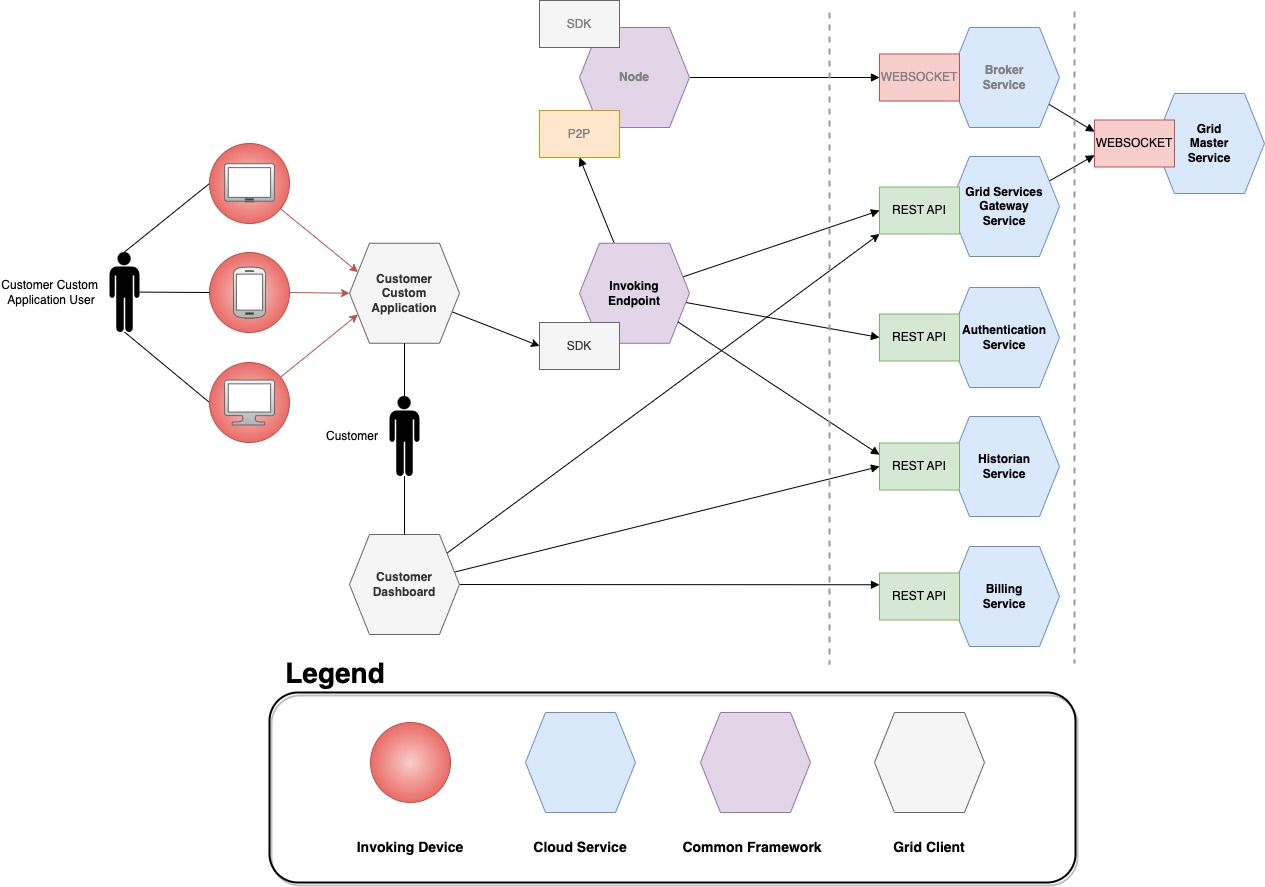
\includegraphics[width=\linewidth]{document/chapters/chapter_6/images/architecture_customer.jpg}
    \caption{Architecture: Customer-relevant view}
    \label{fig:architecture_customer}
\end{figure}

\subsubsection{Invoking Endpoint}
TODO
% High level grid draw.io: something similar to MapReduce but for a general task

\subsubsection{Customer Custom Application}
TODO
% focus on sdk

\subsubsection{Customer Dashboard}
TODO
% Mockups